\documentclass[../../main.tex]{subfiles}
\begin{document}
\section{Cantilever beam} \label{sec:Timo:Cantilever}
Consider a cantilever Timoshenko beam model (Problem T-3 as defined in section \ref{ssec:1D_Model:ModelProblems}). The eigenvalue problem of Problem T-3 is denoted by Problem T-3E. This section serves as an example of the application of the theory from \cite{VV06}.\\

Consider the general solutions of the eigenvalue problem for the three cases $\lambda < \alpha$, $\lambda = \alpha$ and $\lambda > \alpha$. Imposing the boundary conditions $x = 0$ results in the following constants:
\begin{align}
	C = & \frac{\mu(\lambda-\omega^2)}{\omega(\lambda+\mu^2)}A  \  &\textrm{ and } \ D = -B  \ \textrm{ if } \lambda < \alpha \label{A1}\\
	C = & \frac{\omega}{\lambda - \omega^2}A  \  &\textrm{ and } \ D = -B  \ \textrm{ if } \lambda = \alpha \label{A2}\\
	C = & -\frac{\omega(\lambda-\theta^2)}{\theta(\lambda-\omega^2)}A  \  &\textrm{ and } \ D = -B  \ \textrm{ if } \lambda > \alpha \label{A3}
\end{align}
The boundary conditions at $x = 1$ reduces the general solution to the following two-dimensional homogeneous system for each of the three cases.

\begin{align}
	\begin{bmatrix}
		M_{11}(\lambda) & M_{12}(\lambda)\\
		M_{21}(\lambda) & M_{22}(\lambda)
	\end{bmatrix}
	\begin{bmatrix}
		A\\
		B
	\end{bmatrix}
	= 
	\begin{bmatrix}
		0\\
		0
	\end{bmatrix}
\label{eq:Timo:Cantilever:SystemOfEquations}
\end{align}

To obtain non-zero solutions, the determinant of the coefficient matrix $M$ is set to zero, ie. $\textrm{det}(M) = 0$, and is called the frequency equation after simplification. The frequency equations for all three cases is given in [VV06] and is presented below.\\
%freq not defined. freq when simplified and by authors

Case $\lambda < \alpha$:\\
\begin{align}
	\left(\frac{\lambda + \mu^2}{\lambda - \omega^2} + \frac{\lambda - \omega^2}{\lambda + \mu^2} \right) \cosh (\mu) \cos (\omega) + \left(\frac{\omega}{\mu} - \frac{\mu}{\omega}\right) \sinh (\mu) \sin (\omega) - 2 = 0 \label{Freq1}
\end{align}

Case $\lambda = \alpha$:\\
\begin{align}
	\left(\frac{\alpha}{\alpha - \omega^2} + \frac{\alpha - \omega^2}{\alpha} \right) \cos (\omega) + \omega \sin (\omega) - 2 = 0 \label{Freq2}
\end{align}

Case $\lambda > \alpha$:\\
\begin{align}
	\left(\frac{\lambda + \theta^2}{\lambda - \omega^2} + \frac{\lambda - \omega^2}{\lambda + \theta^2} \right) \cos (\theta) \cos (\omega) + \left(\frac{\omega}{\theta} - \frac{\theta}{\omega}\right) \sin (\theta) \sin (\omega) - 2 = 0 \label{Freq3}
\end{align}

Inspection of the system of equations \eqref{eq:Timo:Cantilever:SystemOfEquations}, shows that the coefficient matrix is never zero for the case of the cantilever beam. It follows that all the eigenvalues are simple eigenvalues. This is mentioned in [VV06].

\subsection{Calculating the eigenvalues}
The solutions of the frequency equations \eqref{Freq1} - \eqref{Freq2} can be calculated using simple numerical methods. Using interval division, the eigenvalues are calculated accurate to at least 4 significant digits.
\FloatBarrier
\begin{table}[htbp]
	\centering
	\caption{First 8 eigenvalues, with $\gamma = 0.25$.}
	\begin{tabular}{|c||c|c|c|}
		\hline
		\multicolumn{4}{|c|}{Cantilever Beam Eigenvalues}\\
		\hline
		{i} & {$\alpha = 1200$} & {$\alpha = 4800$} & {$\alpha = 10800$} \\
		\hline
		1     & 0.04043 & 0.01025 & 0.004569 \\
		2     & 1.427 & 0.3914 & 0.1772 \\
		3     & 9.657 & 2.937 & 1.361 \\
		4     & 31.06 & 10.62 & 5.08 \\
		5     & 70.51 & 27.02 & 13.4 \\
		6     & 130.8 & 55.63 & 28.67 \\
		7     & 213.4 & 99.54 & 53.36 \\
		8     & 318.7 & 161.2 & 89.85 \\
		\hline
	\end{tabular}%
	\label{tab:addlabel}%
\end{table}%
\FloatBarrier


\textbf{Remark:} For interval division, the frequency equations are sketched to determine intervals to isolate the solutions. Another method that requires less user involvement is the bisection method. The advantage of the interval method is that the number of solutions within any given interval can be determined visually before the method is applied.

\subsection{Example of mode shapes}
Substituting a calculated eigenvalue $\lambda_k$ back into \eqref{eq:Timo:Cantilever:SystemOfEquations}, the values for $A_k$ and $B_k$ can be calculated by solving the system. But since $\textrm{det}(M) =0$, there are infinity many solutions of $[A_k \ B_k]^T$ for each $k$. So either one of $A_k$ or $B_k$ can be chosen freely and the other is depended on the choice. The modal shapes are sketched below in Figure 4.1 (modal shapes for $u$) and Figure 4.2 (modal shapes for $\phi$) corresponding to the eigenvalue $\lambda_k$ with $A_k = 1$, $\alpha = 1200$ and $\gamma = 0.25$.
\FloatBarrier
\begin{figure}[h!]
	
	\makebox[\textwidth][c]{
		\centering
		\begin{minipage}[b]{0.7\linewidth}
			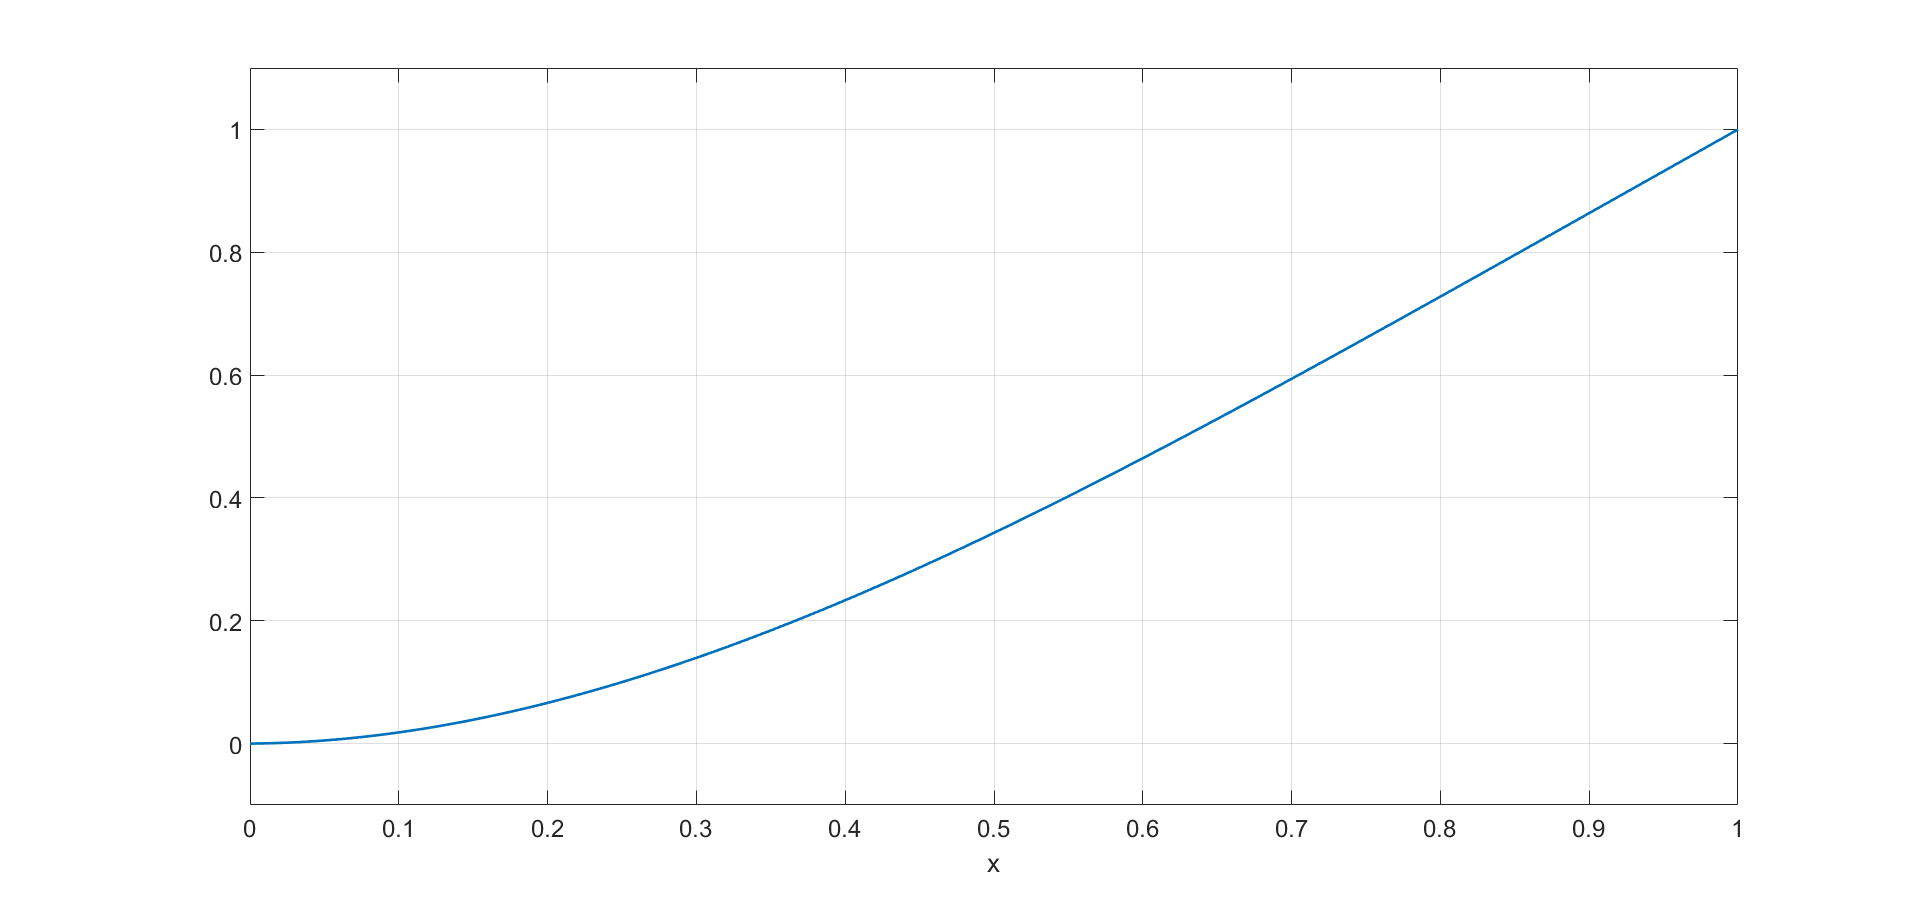
\includegraphics[width=1\linewidth]{Cant1.png}
			\subcaption{ $\lambda_1 = 0.04043$, $B_1 = -1.368$}
			\label{fig:minipage2}
		\end{minipage}
		\begin{minipage}[b]{0.7\linewidth}
			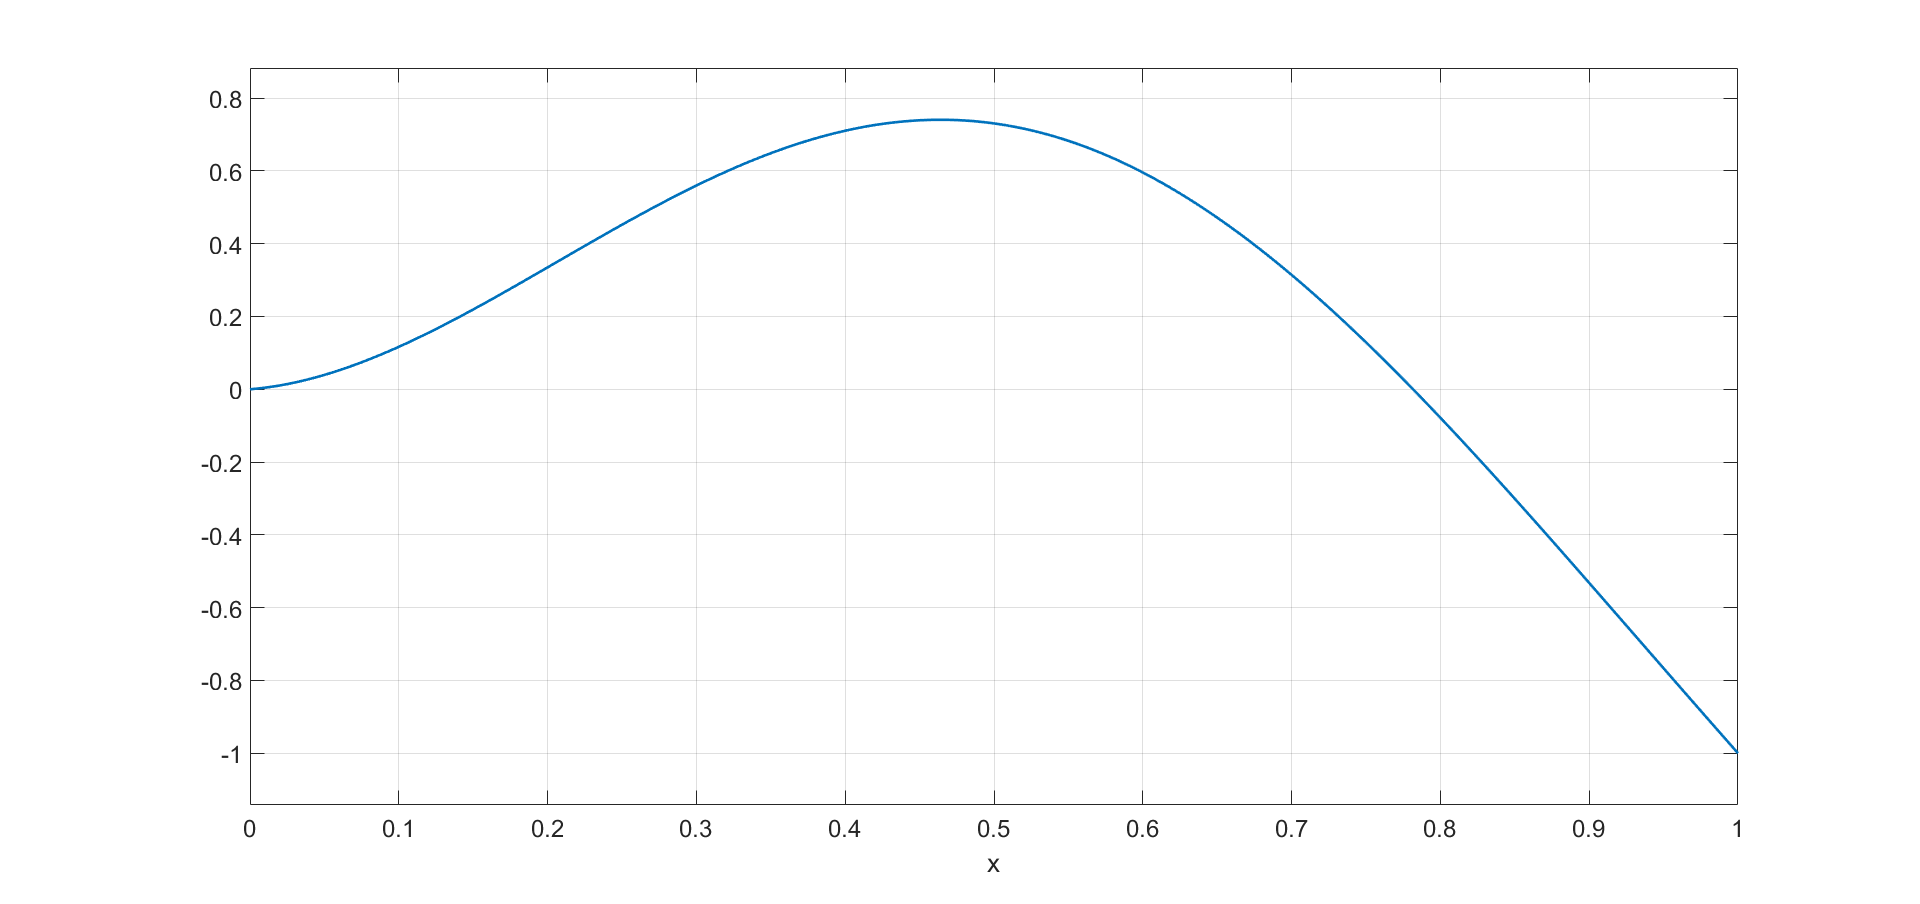
\includegraphics[width=1\linewidth]{Cant2.png}
			\subcaption{$\lambda_2 = 1.427$, $B_2 = -0.9768$}
			\label{fig:minipage1}
		\end{minipage}
	}
	
	\makebox[\textwidth][c]{
		\centering
		\begin{minipage}{.7\textwidth}
			\centering
			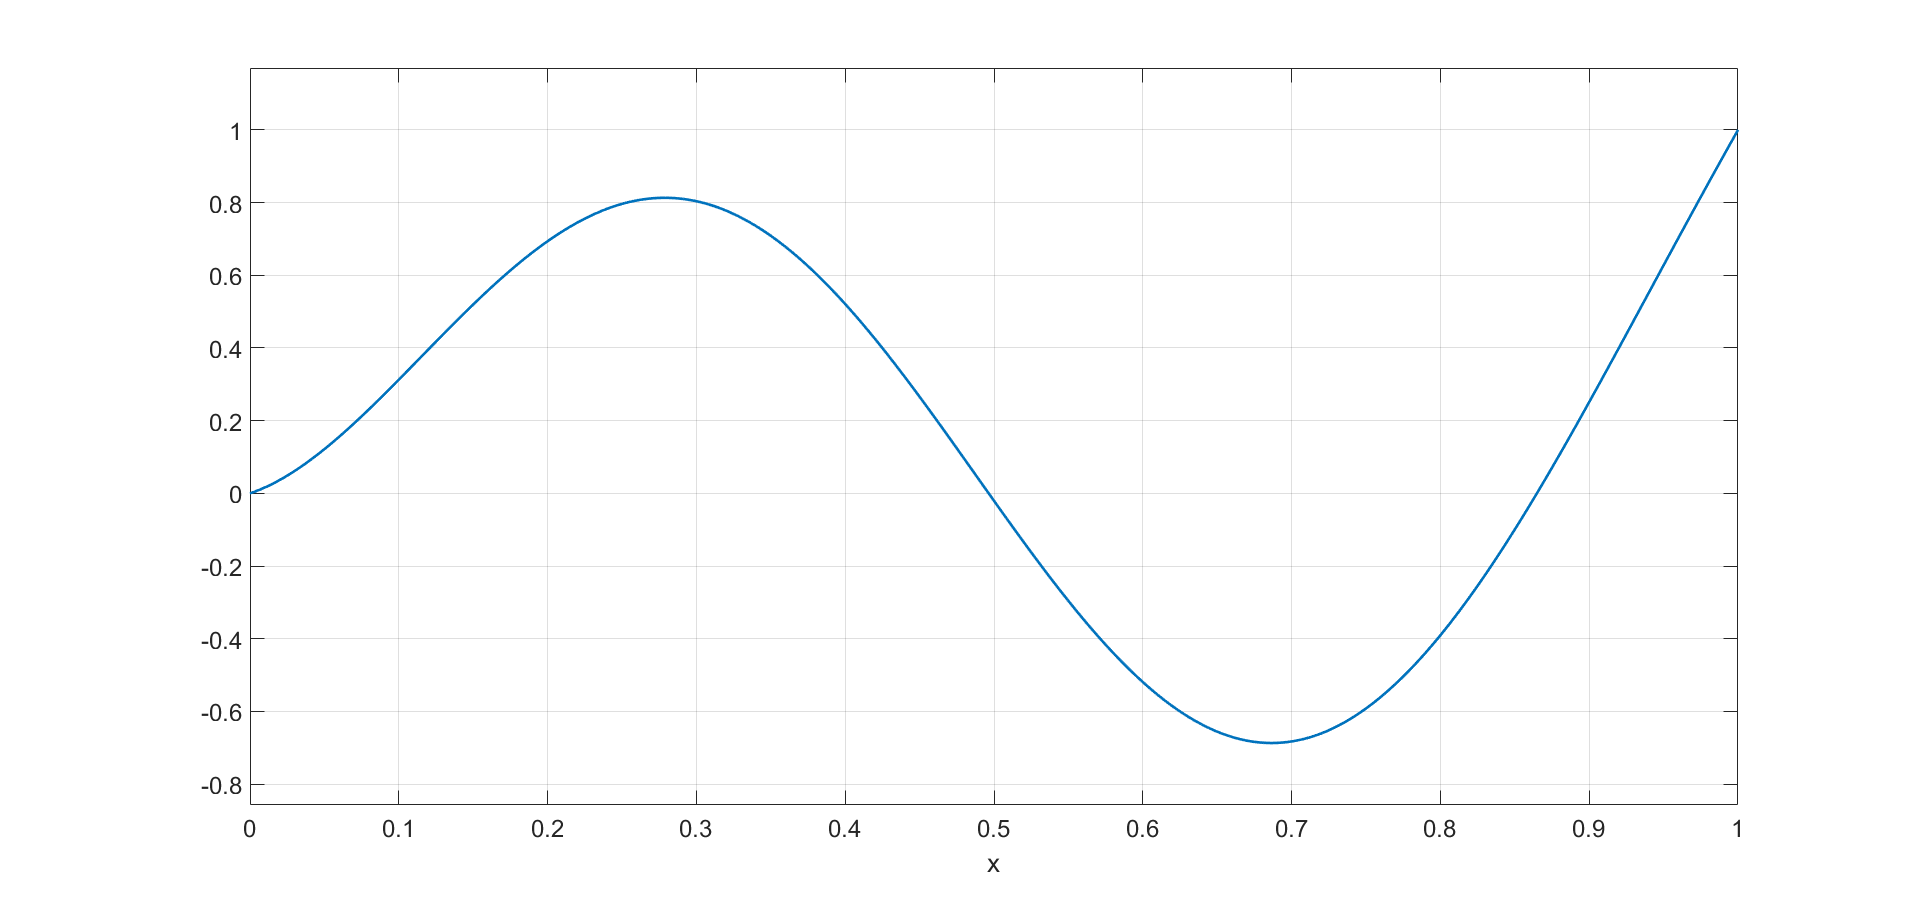
\includegraphics[width=1\linewidth]{Cant3.png}
			\subcaption{$\lambda_3 = 9.657$, $B_3 = -1.002$}
			\label{fig:minipage1}
		\end{minipage}
		\begin{minipage}{.7\textwidth}
			\centering
			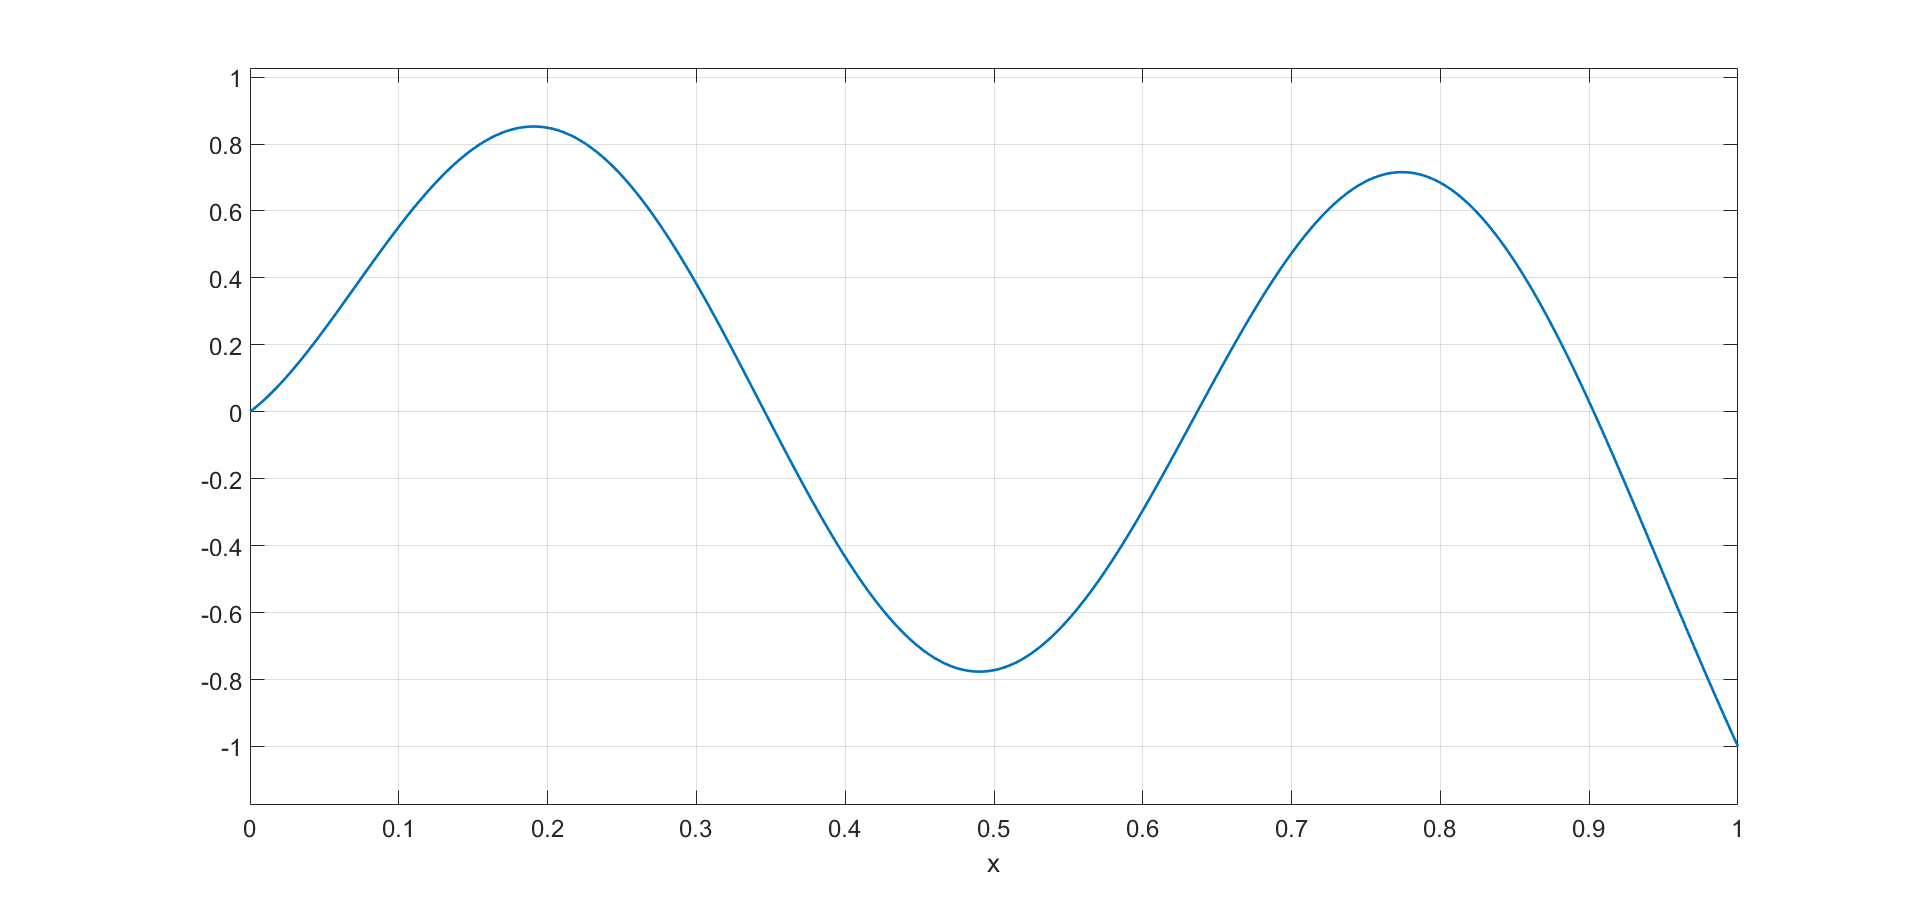
\includegraphics[width=1\linewidth]{Cant4.png}
			\subcaption{$\lambda_4 = 31.06$, $B_4 = -0.9997$}
			\label{fig:minipage2}
		\end{minipage}
	}
	\caption{Sketch of $w$ for the first 4 mode shapes of the cantilever beam. $\alpha = 1200$ and $\gamma = 0.25$ with $A_k = 1$.}
\end{figure}
\FloatBarrier

\begin{figure}[h!]
	
	\makebox[\textwidth][c]{
		\centering
		\begin{minipage}[b]{0.7\linewidth}
			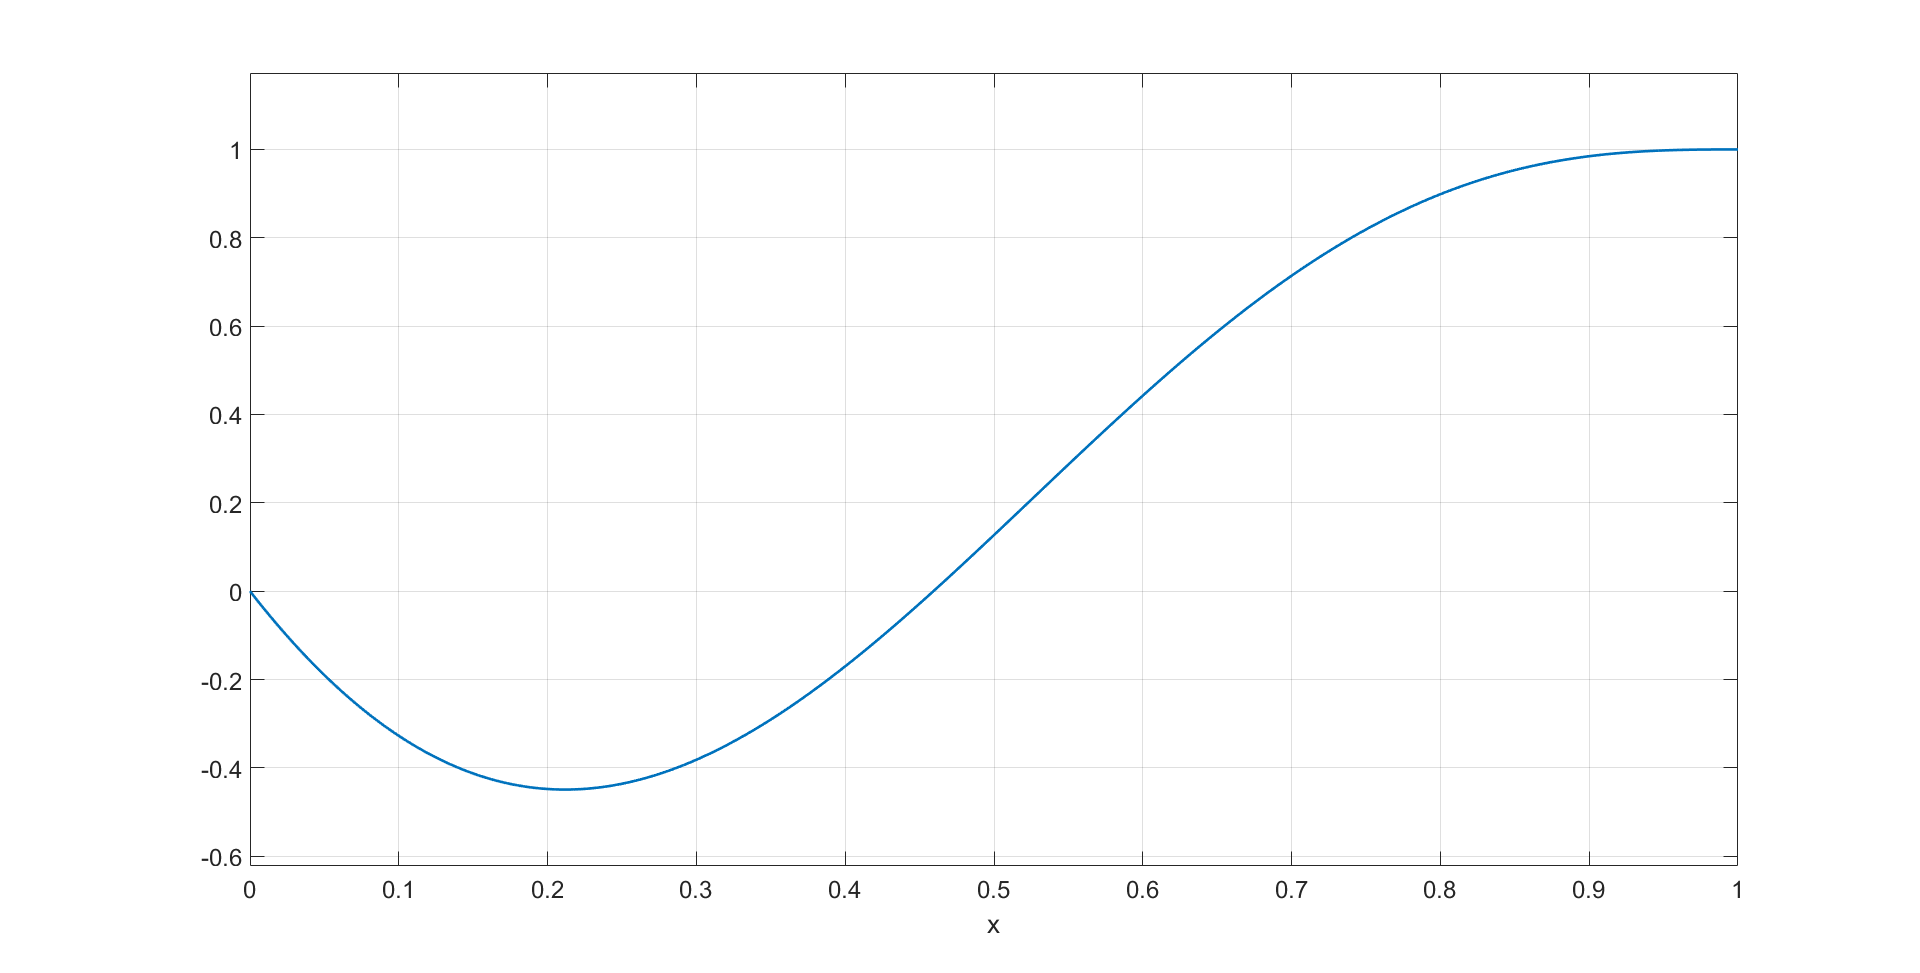
\includegraphics[width=1\linewidth]{Cant21.png}
			\subcaption{ $\lambda_2 = 1.427$, $B_1 = -0.9768$}
			\label{fig:minipage2}
		\end{minipage}
		\begin{minipage}[b]{0.7\linewidth}
			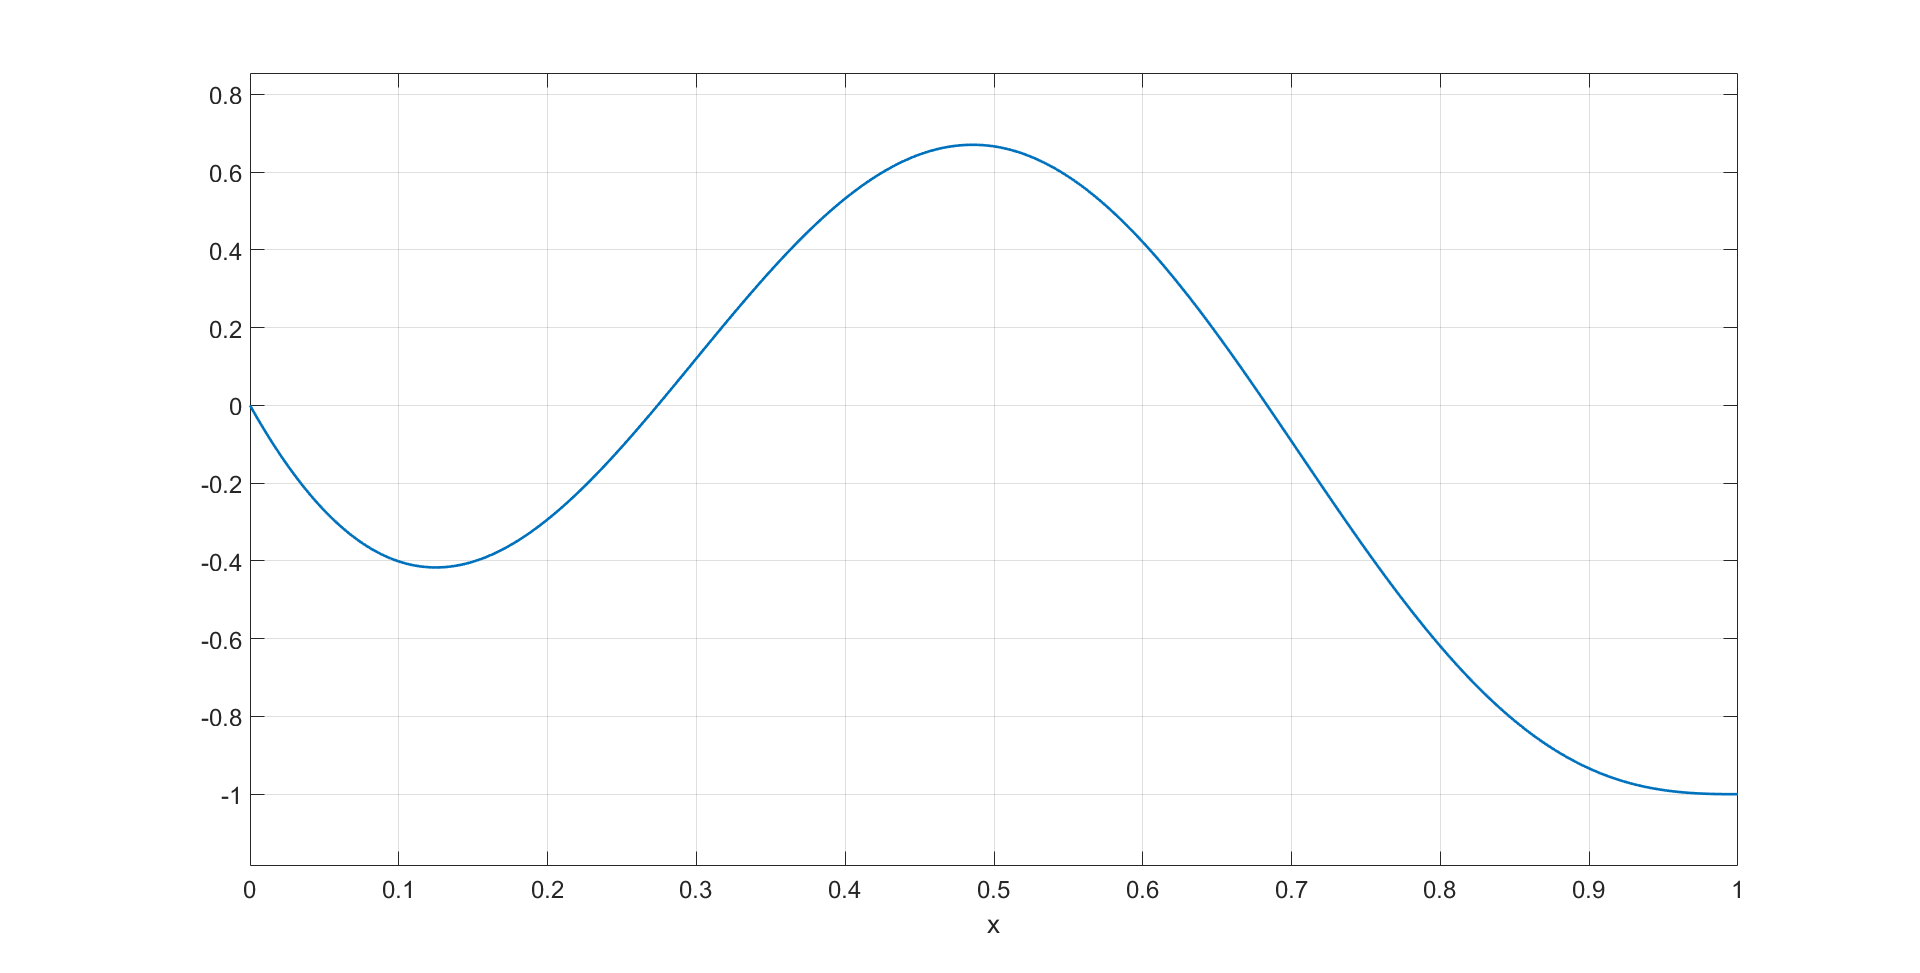
\includegraphics[width=1\linewidth]{Cant31.png}
			\subcaption{$\lambda_3 = 9.657$, $B_2 = -1.002$}
			\label{fig:minipage1}
		\end{minipage}
	}
	
	\caption{Sketch of $\phi$ for mode shapes 2 and 3 of the cantilever beam. $\alpha = 1200$ and $\gamma = 0.25$ with $A_k = 1$.}
\end{figure}

\FloatBarrier
\textbf{Remark:} The sketch of $\phi$ for the first mode shape is similar to the sketch of $w$ and is therefore omitted.\\
\FloatBarrier

The results obtained for the Cantilever beam model are the same as the results in [VV06]. The motivation for this model is Chapter 6. The work of this section will be used for comparisons to a two and three-dimensional cantilever beam model.

\end{document}
